\chapter{Unit and Integration Testing: Frameworks} ha l'obiettivo di far emergere malfunzionamenti derivanti dall'interazione tra due o più moduli o componenti del \textbf{System Under Test} (SUT).

In particolare, serve ad acquisire confidenza che:

\begin{itemize}
    \item esistano le dovute interconnessioni tra i moduli o componenti del SUT;
    \item le interazioni rispettino i \textbf{contratti funzionali} stabiliti dai protocolli o dalle specifiche di interazione.
\end{itemize}

L'assunzione di partenza è che ogni modulo, testato in isolamento, si comporti correttamente. In altre parole, i \textbf{test di unità} devono essere già stati superati.

I test di integrazione possono essere progettati secondo approcci diversi:

\begin{itemize}
    \item \textbf{white-box}, se si conosce il codice dei moduli coinvolti;
    \item \textbf{black-box}, se ci si basa solo sulle specifiche di interazione;
    \item \textbf{misto}, situazione molto frequente nella pratica.
\end{itemize}

\begin{notaprof}
Nella pratica si usano spesso approcci misti. Da un lato serve conoscere l'API esposta, quindi il contratto visibile dall'esterno; dall'altro può essere necessario conoscere alcune meccaniche interne per configurare correttamente l'interazione tra componenti.
\end{notaprof}

Poiché il test di integrazione è spesso incrementale, non sempre tutti i moduli sono disponibili o desiderabili nell'ambiente di test. Per questo motivo si usano \textbf{stub}, \textbf{mock} e \textbf{test driver}.

Uno \textbf{stub} o \textbf{mock} simula il comportamento di un'unità mancante o non considerata nel test. Spesso tale comportamento è semplice, costante o controllato artificialmente.

Un \textbf{test driver} è invece un elemento software che esegue o coordina il test, configurando l'ambiente, preparando le risorse, attivando le interazioni e svolgendo operazioni di clean-up dopo l'esecuzione.

\section{Strategie di integration testing}

Identificare una strategia ottima di integrazione è, in generale, un problema difficile.

\begin{notaslide}
Le slide indicano che la scelta ottima può essere formulata come un problema \textbf{NP-complete}.
\end{notaslide}

Le strategie comuni sono:

\begin{itemize}
    \item \textbf{big bang};
    \item \textbf{top-down};
    \item \textbf{bottom-up}.
\end{itemize}

\begin{figure}[htbp]
    \centering
    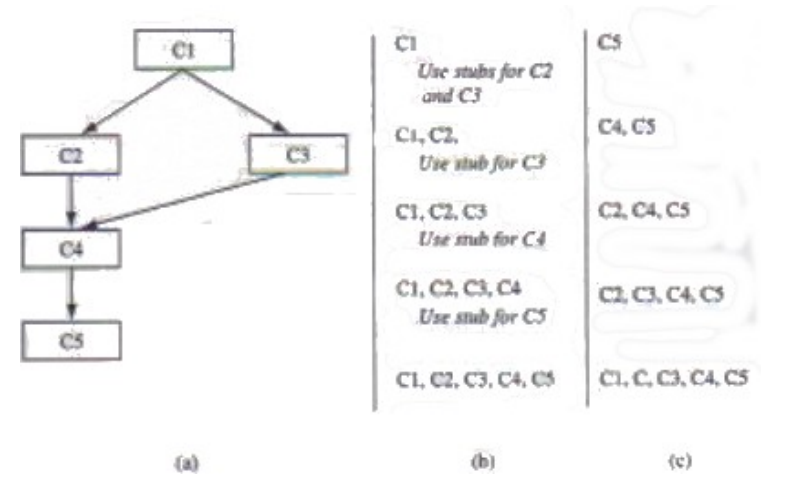
\includegraphics[width=0.72\textwidth]{img/DeAngelis/05_UnitIntegration_Frameworks/slide06}
    \caption{Principali strategie di integration testing. La figura mette a confronto approccio big bang, top-down e bottom-up, evidenziando il ruolo di stub e test driver nel raffinamento progressivo dell'integrazione.}
    \label{fig:lez17-integration-strategies}
\end{figure}

\subsection{Big bang}

La strategia \textbf{big bang} consiste nell'integrare tutte le componenti in un unico passo e testare il sistema risultante.

\begin{notaprof}
È la soluzione più semplice da descrivere, ma spesso è sconsigliata. Se il sistema fallisce dopo aver integrato tutto insieme, diventa molto difficile capire quale interazione abbia causato il problema. Inoltre, più difetti possono mascherarsi a vicenda.
\end{notaprof}

\subsection{Top-down}

La strategia \textbf{top-down} parte dalle interfacce esposte e dalle funzionalità più generali, cioè quelle più vicine ai confini del SUT.

Le sequenze di test sono definite a partire dagli scenari d'uso del sistema. Il raffinamento avviene progressivamente:

\begin{itemize}
    \item sostituendo gli stub con implementazioni reali;
    \item aggiungendo moduli interni via via più dettagliati;
    \item ampliando il sottoinsieme del sistema considerato.
\end{itemize}

\begin{notaslide}
Nel top-down, gli \textbf{stub} simulano comportamenti o funzionalità mancanti dei moduli più profondi.
\end{notaslide}

\begin{notaprof}
Nel top-down si parte dall'alto, cioè dalle funzionalità più visibili, e si scende progressivamente verso i dettagli interni. Gli stub vengono rimpiazzati quando i componenti reali diventano disponibili.
\end{notaprof}

\subsection{Bottom-up}

La strategia \textbf{bottom-up} parte dalle unità elementari, cioè dai componenti più interni o lontani dai bordi del sistema.

In questo caso il raffinamento avviene considerando progressivamente interfacce più generali o parti più periferiche del sistema.

\begin{notaslide}
Nel bottom-up, i \textbf{test driver} simulano il comportamento di moduli o componenti più esterni del sistema. Se alcune funzionalità mancanti devono comunque essere richiamate, possono essere emulate tramite stub.
\end{notaslide}

\subsection{Spiegazione dei diagrammi}

\begin{notaslide}
Il diagramma delle slide mostra una gerarchia di moduli: C1 è il modulo più alto, che interagisce con C2 e C3; questi a loro volta portano verso moduli più interni come C4 e C5.
\end{notaslide}

Nel caso \textbf{top-down}, si parte da C1 e si simulano inizialmente C2 e C3 con stub. Successivamente si introducono C2 e C3 reali, continuando a simulare i moduli più profondi, fino ad arrivare al sistema completo.

Nel caso \textbf{bottom-up}, si parte dai moduli più bassi, ad esempio C5 o C4-C5, usando test driver per simulare i livelli superiori. Si risale poi gradualmente verso C1.

\section{Test di integrazione in sistemi Object-Oriented}

Nei sistemi object-oriented, come quelli Java, i comportamenti emergono spesso dallo scambio di messaggi tra oggetti. Per questo sono utili strumenti che permettano di controllare e simulare tali interazioni.

Gli strumenti principali sono:

\begin{itemize}
    \item \textbf{JUnit}, usato come test driver;
    \item \textbf{Mockito}, usato per stubbing e mocking.
\end{itemize}

\begin{notaprof}
Nei sistemi a oggetti può essere scomodo o costoso costruire manualmente tutte le dipendenze reali. Per esempio, invece di implementare un finto database da zero, si può usare un mock che simula solo il comportamento necessario al test.
\end{notaprof}

\begin{notaslide}
Gli strumenti di test supportano il testing incrementale, permettendo di isolare specifiche interazioni del SUT e di emulare componenti mancanti dell'ambiente.
\end{notaslide}

\section{Mockito}

\textbf{Mockito} è un framework Java per la definizione di stub e mock a supporto dello sviluppo di test di unità e di integrazione.

Mockito permette di:

\begin{itemize}
    \item dichiarare mock e stub;
    \item definire valori di ritorno per operazioni su specifiche istanze;
    \item ridefinire comportamenti in base agli input;
    \item verificare se certe interazioni sono avvenute;
    \item supportare pratiche di sviluppo guidate dai test, come TDD e BDD.
\end{itemize}

\subsection{Costrutti principali}

I principali costrutti di Mockito sono:

\begin{itemize}
    \item \texttt{mock()}: crea un mock programmaticamente;
    \item \texttt{spy()}: crea una spy, cioè un oggetto reale osservabile e parzialmente controllabile;
    \item \texttt{@Mock}: dichiara un mock tramite annotazione;
    \item \texttt{@Spy}: dichiara una spy tramite annotazione;
    \item \texttt{@Captor}: cattura argomenti passati ai mock;
    \item \texttt{@InjectMocks}: inietta automaticamente mock dentro l'oggetto sotto test;
    \item \texttt{thenReturn}: definisce un valore di ritorno fisso;
    \item \texttt{given(...).willReturn(...)}: variante in stile BDD;
    \item \texttt{thenAnswer}: definisce un comportamento dinamico;
    \item \texttt{verify}: controlla che una certa interazione sia avvenuta;
    \item \texttt{then(...).should(...)}: variante BDD della verifica;
    \item \texttt{MockitoJUnitRunner} e \texttt{MockitoJUnit.rule()}: integrazione con JUnit.
\end{itemize}

\begin{notaprof}
Un mock sostituisce il comportamento dell'oggetto configurandone le risposte. Una spy, invece, mantiene il comportamento reale dell'oggetto, ma permette di osservare e verificare le chiamate ai suoi metodi.
\end{notaprof}

\begin{notaprof}
\texttt{@InjectMocks} è utile quando si vuole testare un oggetto reale, ma sostituire automaticamente alcune sue dipendenze interne con mock controllati dal test.
\end{notaprof}

\begin{notaprof}
\texttt{thenAnswer} è utile quando una risposta fissa non basta. Permette di definire una logica dinamica che genera il risultato in base agli argomenti ricevuti.
\end{notaprof}

\subsection{Esempi Mockito}

\begin{notaslide}
Le slide rimandano ai file \texttt{SimpleAgendaTest.java} e \texttt{AgendaTest.java} come esempi di uso di Mockito.
\end{notaslide}

Nel caso di \texttt{SimpleAgendaTest}, il test lavora direttamente su un'interfaccia. Si crea un mock dell'agenda e si configura il comportamento atteso per determinate chiamate.

\begin{notaprof}
Per esempio, si può configurare il mock in modo che, quando viene chiamato \texttt{getAppointment} con una certa data, restituisca una stringa prefissata. Con \texttt{thenAnswer}, invece, si può definire una risposta dinamica basata sull'input.
\end{notaprof}

Nel caso di \texttt{AgendaTest}, si testa un'implementazione reale, come \texttt{MyAgenda}, ma si sostituisce una parte del suo stato interno, ad esempio una \texttt{Map} degli appuntamenti, tramite mock.

\begin{notaprof}
In questo modo il test esercita le API reali di \texttt{MyAgenda}, ma controlla artificialmente una dipendenza interna, rendendo l'ambiente di test più prevedibile.
\end{notaprof}

\section{Maven Surefire Plugin}

Il \textbf{Maven Surefire Plugin} è pensato principalmente per eseguire i \textbf{test di unità}.

Viene attivato durante la fase:

\[
\texttt{test}
\]

del ciclo di build Maven.

Surefire scansiona il progetto Maven cercando test JUnit, tipicamente nella directory:

\[
\texttt{\$\{basedir\}/src/test/}
\]

I test vengono riconosciuti se contengono metodi pubblici annotati con \texttt{@Test} e se le classi rispettano determinati pattern di nomenclatura:

\begin{itemize}
    \item \texttt{Test*};
    \item \texttt{*Test};
    \item \texttt{*Tests};
    \item \texttt{*TestCase}.
\end{itemize}

I report vengono generalmente generati in:

\[
\texttt{\$\{basedir\}/target/surefire-reports/TEST-*.xml}
\]

\begin{notaslide}
Le slide mostrano una configurazione del \texttt{pom.xml} in cui il plugin \texttt{maven-surefire-plugin} è dichiarato sotto \texttt{pluginManagement}. È inoltre mostrata la dipendenza da JUnit con \texttt{scope} impostato a \texttt{test}.
\end{notaslide}

\section{Maven Failsafe Plugin}

Il \textbf{Maven Failsafe Plugin} è pensato per eseguire i \textbf{test di integrazione}.

Viene attivato durante le fasi:

\[
\texttt{integration-test}
\quad \text{e} \quad
\texttt{verify}
\]

Failsafe è utile quando i test richiedono attività più complesse, come:

\begin{itemize}
    \item build di più moduli Maven;
    \item configurazione di un ambiente dedicato;
    \item avvio di container applicativi, come Tomcat o Jetty;
    \item deploy e lancio di servizi o moduli;
    \item clean-up e teardown dell'ambiente dopo l'esecuzione.
\end{itemize}

Failsafe riconosce per default classi di test con pattern:

\begin{itemize}
    \item \texttt{IT*};
    \item \texttt{*IT};
    \item \texttt{*ITCase}.
\end{itemize}

I report vengono generalmente generati in:

\[
\texttt{\$\{basedir\}/target/failsafe-reports/failsafe-summary.xml}
\]

\begin{notaslide}
Le slide mostrano una configurazione del \texttt{pom.xml} in cui il plugin \texttt{maven-failsafe-plugin} associa i goal \texttt{integration-test} e \texttt{verify} all'interno della sezione \texttt{executions}.
\end{notaslide}

\section{Surefire vs Failsafe}

La distinzione principale è:

\begin{itemize}
    \item \textbf{Surefire}: esegue unit test nella fase \texttt{test};
    \item \textbf{Failsafe}: esegue integration test nelle fasi \texttt{integration-test} e \texttt{verify}.
\end{itemize}

\begin{figure}[htbp]
    \centering
    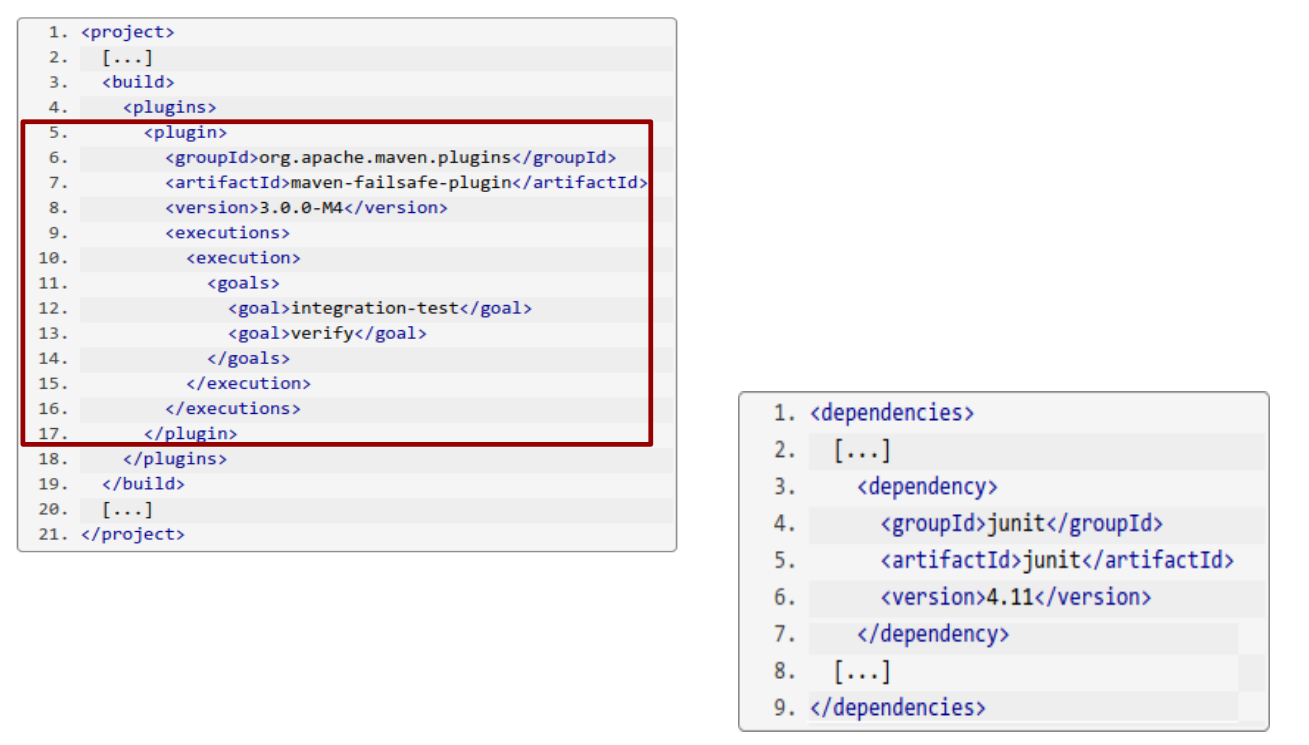
\includegraphics[width=0.72\textwidth]{img/DeAngelis/05_UnitIntegration_Frameworks/slide23}
    \caption{Configurazione del Maven Failsafe Plugin per l'esecuzione dei test di integrazione durante le fasi \texttt{integration-test} e \texttt{verify} del ciclo di build Maven.}
    \label{fig:lez17-maven-failsafe}
\end{figure}

\begin{notaprof}
Quando si esegue \texttt{mvn test}, Maven attiva i test gestiti da Surefire. Quando si esegue \texttt{mvn verify}, Maven arriva anche alle fasi pensate per i test di integrazione e può quindi attivare Failsafe.
\end{notaprof}

Separare unit test e integration test è importante perché hanno costi e scopi diversi. I test di unità dovrebbero essere rapidi e isolati, mentre i test di integrazione possono richiedere ambienti più pesanti, moduli multipli, servizi esterni o container.

\begin{notaesame}
Chiamare un integration test con un nome compatibile con Surefire, ad esempio \texttt{PippoTest.java}, può farlo eseguire nella fase sbagliata. Per i test di integrazione conviene usare pattern come \texttt{*IT.java}.
\end{notaesame}

\section{Raccomandazioni per il progetto}

\begin{notaesame}
Nel progetto è fortemente consigliato sperimentare la progettazione e realizzazione di test di unità associandoli al processo di Continuous Integration tramite Maven Surefire.
\end{notaesame}

\begin{notaesame}
È inoltre consigliato progettare e realizzare test di integrazione associandoli alla Continuous Integration tramite Maven Failsafe.
\end{notaesame}

\begin{notaesame}
Mockito dovrebbe essere usato per simulare componenti e dipendenze sia nei test di unità sia nei test di integrazione.
\end{notaesame}

Errori comuni da evitare:

\begin{itemize}
    \item usare nomi di test non conformi ai pattern riconosciuti da Maven;
    \item inserire integration test complessi in Surefire senza setup e teardown adeguati;
    \item scrivere test senza \texttt{assert} o senza \texttt{verify};
    \item abusare di matcher troppo generici, come \texttt{any()}, indebolendo l'oracolo del test;
    \item confondere il test driver con il SUT;
    \item testare lo stub o il mock invece dell'unità reale sotto test.
\end{itemize}